\documentclass[12pt,a4paper]{article}

\usepackage[in, plain]{fullpage}
\usepackage{array}
%\usepackage{../../../pas-math}
\usepackage{../../../moncours2}




\date{}
\title{\textcircled{{\normalsize{6}}} Proportionnalité}

\graphicspath{{./img/}}


%\toggletrue{eleve}
%\toggletrue{dys}

%\rfoot{Page \thepage}
\begin{document}

\maketitle






\begin{myobj}
	\begin{itemize}
		
		\item Construire le symétrique d’un point ou d'une figure par rapport à une droite à la main où à l’aide d’un logiciel;
		\item Construire le symétrique d’un point ou d'une figure par rapport à un point, à la main où à l’aide d’un logiciel;
		\item Utiliser les propriétés de la symétrie axiale ou centrale;
		\item Identifier des symétries dans des figures.		
	\end{itemize}
\end{myobj}

\begin{mycomp}
	\begin{itemize}
		\item \kw{Chercher (Ch2)} :  s’engager    dans    une    démarche    scientifique, observer, questionner, manipuler, expérimenter (sur une feuille de papier, avec des objets, à l’aide de logiciels), émettre des hypothèses, chercher des exemples ou des contre-exemples, simplifier ou particulariser une situation, émettre une conjecture ;
		\item \kw{Raisonner (Ra3)} :  démontrer : utiliser un raisonnement logique et des règles établies (propriétés, théorèmes, formules) pour parvenir à une conclusion ;
		\item \kw{Communiquer (Co2)} :  expliquer à l’oral ou à l’écrit (sa démarche, son raisonnement, un calcul, un protocole   de   construction   géométrique, un algorithme), comprendre les explications d’un autre et argumenter dans l’échange ; 
		
	\end{itemize}
\end{mycomp}





%\section{Rappel}

\section{Tableau de proportionnalité}

\begin{mydefs}
	
	\iftoggle{eleve}{%
		\begin{itemize}
			\item Un \hrulefill
			
			\vspace*{0.2cm}
			\hrulefill
			
			\vspace*{0.2cm}
			\hrulefill
			
			\vspace*{0.2cm}
			\hrulefill
			
			
			\item \vspace*{0.2cm}
			\hrulefill
		\end{itemize}
	}{%
		\begin{itemize}
			\item Un tableau a deux lignes est un \kw{tableau de proportionnalité} si on peut calculer les nombres de la deuxième lignes sont obtenues en multipliant ceux de la première \kw{par un même nombre}.
			
			\item Ce nombre est le \kw{coefficient de proportionnalité}.
		\end{itemize}
	}
	
	
	
\end{mydefs}


\begin{mymeth}
	
	\iftoggle{eleve}{%
		Pour \hrulefill
		
		\vspace*{0.2cm}
		\hrulefill
		
		\vspace*{0.2cm}
		\hrulefill
		
		
		

	}{%
		Pour identifier une situation de proportionnalité, on calcule les quotients des nombres de la seconde ligne par ceux de la première ligne. 
		Il y a proportionnalité si c'est toujours le même.
	}
	
	
	
\end{mymeth}

\begin{myex}
	
		Ce tableau présente le prix de différentes masses de cerises :
		
	
	
\iftoggle{eleve}{%
	
	\begin{center}
		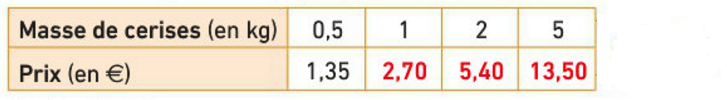
\includegraphics[scale=0.6]{tb_prop1-2}
	\end{center}

	\vspace*{0.2cm}
	\hrulefill
	
	\vspace*{0.2cm}
	\hrulefill
	
	\vspace*{0.2cm}
	\hrulefill
}{%
	\begin{center}
		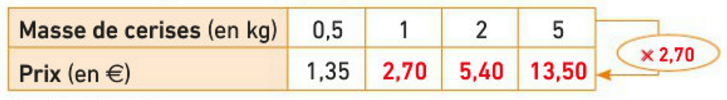
\includegraphics[scale=0.6]{tb_prop1}
	\end{center}

	$\num{1,35} \div \num{0.5} = \num{2,70} \div 1 = \num{5.40} \div 2 = \num{13,50} \div 5 = \num{2.70} $, ce tableau est un tableau de proportionnalité.
	
	Le coefficient de proportionnalité est \num{2.70}.
	
}
	
\end{myex}	

%\begin{myex}	
%		Dans ce tableau on a reporté le nombre de cotés de certains polygones et leur nombre de diagonales.
%		
%		\begin{center}
%			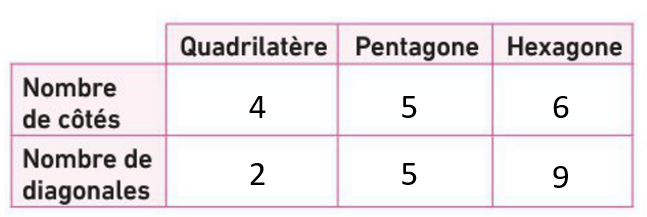
\includegraphics[scale=0.5]{tab2}
%		\end{center}
%	
%		$2 \div 4 = \num{0.5}$, $5 \div 5 = 1$, donc le nombre de côtés d'un polygone n'est pas proportionnel à son nombre de diagonales.	
%	
%\end{myex}
%
\section{Compléter un tableau de proportionnalité}

\begin{mymeth}
	On veut remplir le tableau de proportionnalité suivant :
	
	\begin{center}
		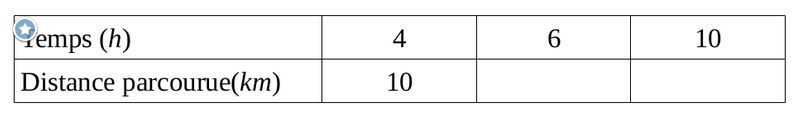
\includegraphics[scale=0.5]{tab3_1}
	\end{center}
\end{mymeth}

\vspace*{-0.5cm}

\subsection{Avec le coefficient de proportionnalité}

%\begin{mymeth}

\iftoggle{eleve}{%
	
	\vspace*{0.2cm} 
	\hrulefill
	
	
	\vspace*{0.2cm} 
	\hrulefill
	
	
	\begin{center}
		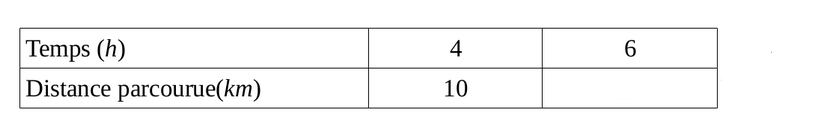
\includegraphics[scale=0.5]{tab3_3-2}
	\end{center}
}{%
	On calcule le coefficient : $10 \div 4 = \num{2.5} $.
	
	Donc  $6 \times \num{2.5} = 15$.
	
	
	\begin{center}
		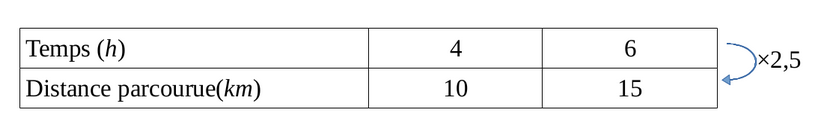
\includegraphics[scale=0.5]{tab3_3}
	\end{center}
}
	
%\end{mymeth}



\vspace*{-0.5cm}

\subsection{En utilisant les propriétés de la proportionnalité}

\begin{myprop}
	
	\iftoggle{eleve}{%
		\vspace*{0.2cm} 
		\hrulefill
		
		\begin{itemize}
			\item \vspace*{0.2cm} 
			\hrulefill
			
			\item 
			\vspace*{0.2cm} 
			\hrulefill
		\end{itemize}
	}{%
		Dans un tableau de proportionnalité, on peut :
		\begin{itemize}
			\item multiplier/diviser une colonne par un nombre;
			\item ajouter/soustraire des colonnes entre elles.
		\end{itemize}
	}
	
	
	
\end{myprop}
%

%\begin{mymeth}
\iftoggle{eleve}{%
	\vspace*{0.2cm} 
	\hrulefill
	
	\vspace*{0.2cm} 
	\hrulefill
	\begin{center}
		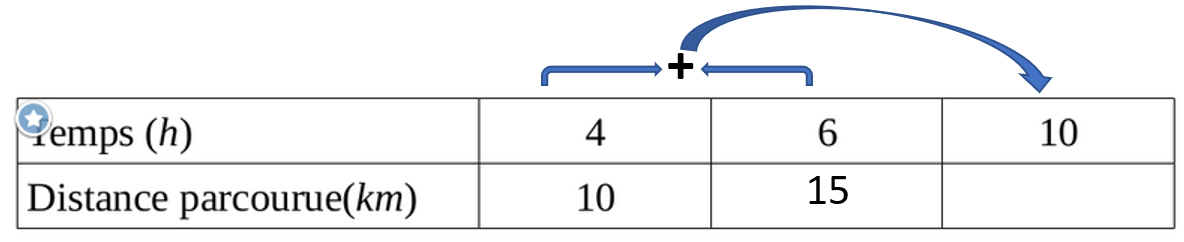
\includegraphics[scale=0.35]{tab3_4-2}
	\end{center}
}{%
	On parcourt 10 km en 4 heures et 15 en 6 heures.
	
	Donc en 10 heures on parcourt 25 km (10 + 15) .
	\begin{center}
		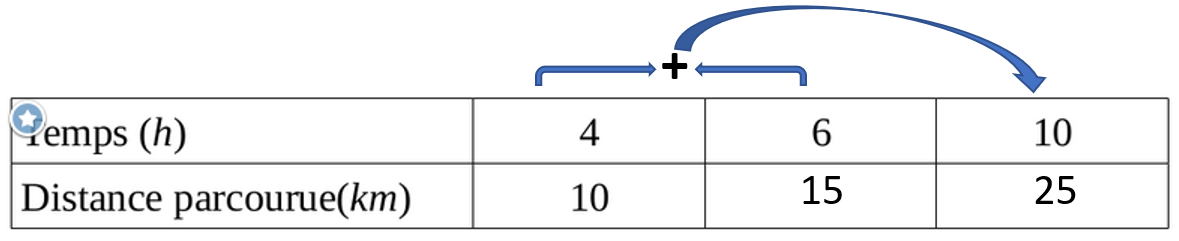
\includegraphics[scale=0.35]{tab3_4}
	\end{center}
}
	
%\end{mymeth}

\vspace*{-0.5cm}

\subsection{Par passage à l'unité}


%\begin{mymeth}

\iftoggle{eleve}{%
	\vspace*{0.2cm} 
	\hrulefill
	
	\vspace*{0.2cm} 
	\hrulefill
	
	\vspace*{0.2cm} 
	\hrulefill
	
	
	
	\begin{center}
		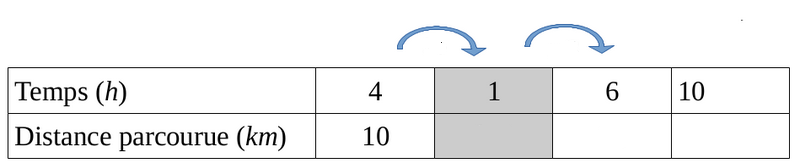
\includegraphics[scale=0.5]{tab3_2-2}
	\end{center}
}{%
	En 4 heures, nous parcourons 10 km.
	
	En 1 heure, nous parcourrons donc $10 \div 4 = \num{2.5}$ km.
	
	En 6 heures, nous parcourrons $\num{2.5} \times 6 = 15 $km.
	
	
	
	\begin{center}
		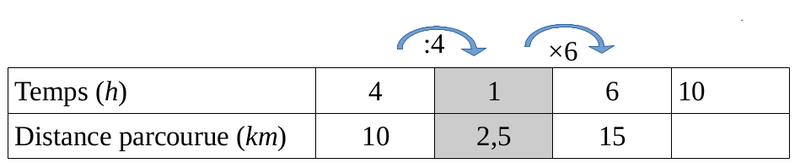
\includegraphics[scale=0.5]{tab3_2}
	\end{center}
}

%\end{mymeth}
%\section{Pourcentages}
%
%\subsection{Appliquer un pourcentage}
%
%\begin{mydef}
%	Un pourcentage traduit une situation de proportionnalité. 
%
%	Un pourcentage est une proportion exprimée sur un total de 100 (de dénominateur égal à 100).
%	
%\end{mydef}
%
%\begin{myex}
%	<<Dans une confiture, il y a 60 \% de fruits>>
%	\begin{itemize}
%		\item La masse de fruits est proportionnelle à la masse totale de confiture.
%		\item[$\Rightarrow$] Il y a 60g de fruits pour 100g de confiture.
%	\end{itemize}
%\end{myex}
%
%
%\begin{myprop}
%	$P$ est un nombre positif.
%	
%	Pour calculer $P\% $ d'une quantité, on multiplie cette quantité par $\frac{P}{100}$.
%\end{myprop}
%
%
%\begin{myex}
%	Calculer $20 \% $ de 50 revient à multiplier 50 par $\frac{20}{100}$ :
%	
%	\begin{equation*}
%		50 \times \dfrac{20}{100} = 50 \times \num{0.2} = 10
%	\end{equation*}
%	
%	
%	$20 \% $ de 50  vaut 10.
%\end{myex}
%
%\subsection{Calculer un taux de pourcentage}
%
%
%\begin{myex}
%	Dans un collège, il y a 800 élèves et 200 sont externes. Quel est le pourcentage d'externes ?\\
%	
%	
%		\begin{tabular}{|l|l|l|}
%			\hline
%			Nombre d'externes & 200 & $P$ \\ \hline
%			Nombre d'élèves   & 800 & 100 \\ \hline
%		\end{tabular}
%	
%	\vspace*{0.5cm}
%
%	
%	Ce tableau est un tableau de proportionnalité. Le coefficient de proportionnalité est 4 ($800 \div 200$).
%	
%	Calcul de $P$ : $100 \div 4 = 25$.\\
%	
%	 Il y a $25 \%$ d'externes.
%\end{myex}
%\section{Notion d'échelle}
%
%\begin{mydef}
%	\begin{itemize}
%		\item 	Sur un plan à \kw{l'échelle}, les longueurs sur le plan sont proportionnelles aux longueurs dans la réalité.
%		
%		\item  L'échelle d'un plan est  est le quotient de la longueur sur le plan par la longueur réelle correspondante, lorsque ces longueurs sont exprimées dans la même unité.
%	\end{itemize}
%
%\end{mydef}
%
%\begin{myexs}
%	\begin{enumerate}
%		\item Un plan est à l'échelle $ 1 / \num{2000}$. Cela signifie que 1 cm sur le plan représente 20 m (\num{2000} cm) dans la réalité. Les longueurs du plan sont 2000 fois plus petites que les longueurs réelles.
%		
%		
%		\item Un schéma est à l'échelle 50. Cela signifie que 1 cm sur le schéma représente \num{0.02} cm dans la réalité. Les longueurs du plan sont 50 fois plus grandes que les longueurs réelles.
%		
%		
%		\item Sur une carte, 3 cm représentent  12 km dans la réalité. Quelle est l'échelle de la carte ?
%		
%		12 km = \num{1200000} cm.
%		\begin{equation*}
%		\dfrac{3}{\num{1200000}} = \dfrac{1}{\num{400000}}
%		\end{equation*}
%		
%		L'échelle de cette carte est $1 / \num{400000}$.
%	\end{enumerate}
%\end{myexs}
%
%\begin{myrems}
%	\begin{itemize}
%		\item Une échelle n'a pas d'unité.
%		\item L'échelle d'un plan est est le nombre par lequel on multiplie les longueurs réelles pour obtenir les longueurs sur le plan, dans la même unité.
%	\end{itemize}
%\end{myrems}
\end{document}

